% $File: expr.tex
% $Date: Wed Jun 10 00:42:45 2015 +0800
% $Author: jiakai <jia.kai66@gmail.com>

\chapter{评测方法与实验\label{chap:expr}}
本章首先提出一种评测方法,其完全基于对某器官的分割标注,
无需基于其它的柔性匹配算法,也无需显式计算两个标注间的点对应关系,
可以直接评价特征的优劣,简便高效。随后本章介绍实验所用数据集,
并报告基于该评测方法的实验结果。

\section{评测方法}
% f{{{
在实际应用中,往往难以有单一可靠的方法直接评判特征优劣,
而是需要有一个依赖某特征的具体任务,
并通过该特征在该任务上的表现来间接反应特征优劣。
例如,SIFT特征最早被用于物体识别\cite{lowe1999object},
层叠卷积ISA被用于动作识别\cite{le2011learning}、
大脑MRI扫描的柔性配准\cite{wu2013unsupervised}等。
然而,如果任务过于复杂,
结果往往会受到任务相关的具体算法的影响。
例如在Guorong Wu的工作\cite{wu2013unsupervised}中,
作者的评测过程依赖于第三方软件的预处理,
而且发现换用ISA特征后在Demons算法上的配准性能反而变差了,
虽然作者表示这是由于实验过程带来的一些不公平造成的,
但客观而言在这种复杂的环境下确实更难分离出特征本身在最终性能里的贡献。
因此,在本节中,我们将提出一个新的简单而普适的方法来评测特征性能,
以免结果受到过于复杂的任务相关算法的影响。
简单而言,该方法基于人工标定的器官分割掩膜,在不需要具体点对应关系的情况下,
来评价一个特征在测试图像里寻找参考图像中某个点的准确度。

\subsection{基于器官分割标注的曲面匹配}
我们的评测方法要求数据提供对某个器官的分割标注,
例如在本文中我们使用SLIVER07中的肝脏分割标注。
在本小节中,我们将介绍基于大量带器官分割标注的训练数据,
在单个测试图像上寻找某个曲面的方法。为此,我们先定义单点匹配,
并将其扩展到曲面。

\subsubsection{单点匹配}
基于分割标注,我们对每个点都定义{\bf 边界距离},
并基于边界距离来判断单点是否匹配成功。

我们假设器官分割掩膜以二值3D图像$\vec{M}$的形式提供,
$\vec{M}$中某点值为$1$时表示对应点属于目标器官,为$0$时表示不属于目标器官。
对于每个点$(i, j, k)$,定义
\begin{eqnarray}
    N(i, j, k) &=& \prod_{
        \max(\abs{x}, \abs{y}, \abs{z}) = 1}
        M(i + x, j + y, k + z)
\end{eqnarray}
$N(i, j, k)$表示了与$(i, j, k)$相邻的点中是否有不属于目标器官的点。
于是可定义边界点集为:
\begin{eqnarray}
    \partial M &=& \left\{\,\vec{p} : M(\vec{p}) = 1\,\text{且}\,
        N(\vec{p}) = 0\,\right\}
\end{eqnarray}

把每个点看作无向图的顶点,同时在几何上看作一个单位立方体,
对于有公共顶点或公共边的两点间连一条权值为$1$的边,
于是对任意两点$\vec{p}, \vec{q}$,其间存在最短路,
距离记作$s(\vec{p}, \vec{q})$。
对每个点$\vec{p}$,可定义无符号边界距离$D(\vec{p})$和边界距离$d(\vec{p})$:
\begin{eqnarray}
    D(\vec{p}) &=& \min_{\vec{q} \in \partial M} s(\vec{p}, \vec{q}) \\
    d(\vec{p}) &=& (2M(\vec{p})-1)D(\vec{p})
\end{eqnarray}
在涉及多个图像如$\vec{M_1}$、$\vec{M_2}$时,
我们通过脚注形式来区分各自的边界距离:
$d_{\vec{M_1}}(\vec{p})$、$d_{\vec{M_2}}(\vec{q})$。

对于参考图像$\vec{R}$上的某点$\vec{p}$及其特征$\vec{f(p)}$,
我们在测试图像$\vec{T}$上寻找特征距离最小的点$\vec{q}$,
称$\vec{q}$为$\vec{p}$的匹配点,
如果还有$\abs{d_{\vec{R}}(\vec{p}) - d_{\vec{T}}(\vec{q})} \le \theta$,
则认为匹配成功,其中$\theta$为容忍的距离误差,本文中均取$1$。
为了在特征上快速、精确地寻找匹配点,即特征空间上的最近邻,
我们把两两特征间的距离计算转换成矩阵乘法并在GPU上运行。

\subsubsection{曲面匹配\label{sec:expr:match}}
上述单点匹配的判别方法,易受各种随机因素的影响,
在这里我们将其扩展到曲面匹配以提高鲁棒性。

首先根据边界距离,对器官分割标注$\vec{M}$定义参考曲面:
\begin{eqnarray}
    \hat{\vec{M}} &=& \left\{ \vec{p} : d_{\vec{M}}(\vec{p}) = d_0 \right\}
\end{eqnarray}
在本文中,取参考曲面为边界稍靠内的曲面,取$d_0=2$,
这样的一个好处是所有可匹配点的距离在$[1, 3]$间,也都在目标器官内部。

假设我们有$N$个训练数据$\vec{M_1},\cdots,\vec{M_N}$,
我们在$\hat{\vec{M_1}},\cdots,\hat{\vec{M_N}}$上各均匀选取$T$个点,
并在测试图像的上寻找这$NT$个点的匹配点。
为了防止特征只注重了很明显的局部特点而导致匹配点过于集中,
我们把测试图像分成了若干个小方格,每个的大小为$k\times k \times k$,
对于落入同一方格的匹配点,只记录其中距离最小的点,
匹配精确度定义为这些剩下的点中成功匹配的点数占剩下的点总数的比例。
在本文的实验中,均取$T=3000, k=2$。


\subsection{ROC曲线}
基于\secref{expr:match}中针对单个测试图像的曲面匹配方法,
在本小节中我们给出其ROC曲线绘制的方法,以及多个测试图像的整体评分方法。

假设有$M$个测试图像,固定特征距离阈值$\theta$,对每个测试图像,
仅保留$\theta$以下的匹配点,则此时可以得到$(a_1^{(\theta)},
t_1^{(\theta)}),\cdots,(a_M^{(\theta)}, t_M^{(\theta)})$共$M$个二元组,
$a_i^{(\theta)}$表示所有训练图像在第$i$个测试图像上
距离不超过$\theta$的匹配点中成功匹配的比例,即$\theta$限制下的匹配精确度;
$t_i^{(\theta)}$表示这些匹配点占所有训练图像的参考曲面上选中的点的比例,
沿用上节记号,则这些选中的点的总数为$NT$,
$t_i^{(\theta)}$就是$\theta$限制下总匹配点数与$NT$之商。
记$a^{(\theta)}$、$s^{(\theta)}$分别为
$a_1^{(\theta)},\cdots,a_M^{(\theta)}$的均值和方差,
$t^{(\theta)}$为$t_1^{(\theta)},\cdots,t_M^{(\theta)}$的均值,
显然$t^{(\theta)}$随着$\theta$增加是单调不下降的。
遍历$\theta$取值,
将所有$(t^{(\theta)}, a^{(\theta)})$对应的平面点连接起来,
就得到了ROC曲线,
同时可以作出$a^{(\theta)} \pm s^{(\theta)}$的对应区域来反应评测的准确度。
在本文的ROC曲线中,我们把$a^{(\theta)}$称为精确度(precision),
$t^{(\theta)}$称为顶峰比(top ratio)。

\figref{expr:match}展示了在阈值限制下匹配点分布的变化。
可以发现,当限制阈值后,输出的都是该模型比较确信的点,
这些点更靠近如肝肺交界处等有强边缘特征的区域,
匹配精确度能有较大提高。
为了防止顶峰比较低时仅考虑集中于强边缘区域的匹配点而影响对整体性能评价,
我们仅考虑顶峰比在区间$[0.05, 1]$范围内的曲线。

\begin{figure}[H]
    {
        \addplot{res/expr-match/48.2.png}
        \addplot{res/expr-match/80.1.png}
        \caption{限制阈值导致匹配点分布的变化}
        \label{fig:expr:match}
    }
    \footnotesize
    这两张图均通过在x轴上按4像素为步长切片绘制。
    其中彩色标注的区域是人工标注的肝脏区域,绿色点为成功匹配点,
    蓝色点为失败匹配点,蓝色、绿色颜色越亮,则表示匹配的特征距离越小。
    为方便查看,每个点用原始点为中心的$5\times 5 \times 5$立方体来表示,
    因此在某些切片上的一些成功匹配点看起来离参考曲面很远,
    其实是来自曲率变化剧烈的区域的其它(未在此绘制的)切片。

    上图绘制了所有匹配点,顶峰比为$0.568$,匹配精确度为$48.2\%$;
    下图限制了阈值,顶峰比为$0.078$,匹配精确度为$80.1\%$。
\end{figure}

\figref{expr:curve:ISA}给出了一条这样的ROC曲线,
其中每个线条后的半透明背景反映了$s^{(\theta)}$的大小。
比较两条曲线时,精确度越高、精确度的方差越小、
顶峰比越高,则对应的特征的性能越好。
为了比较两条曲线,我们可以用AUC(Area Under Curve, 曲线下面积)
及平均精确度两个指标。
AUC定义为曲线的精确度对顶峰比的定积分值,
平均精确度为AUC除以顶峰比的最大、最小值之差。
在本文的ROC曲线中,各曲线名称后的括号里注明的数字是平均精确度。

% f}}}

\section{实验数据集}
% f{{{
本文的实验均采用SLIVER07\cite{heimann2009comparison}
所提供的腹腔CT扫描数据及肝脏标注。
SLIVER07是一次肝脏分割的比赛,提供了20个训练数据,
由于数据损坏等原因我们仅成功解压出其中的18个数据,
并随机选取其中12个作为训练数据,6个作为测试数据。
先对这18个数据按如下步骤预处理:
\begin{enumerate}
    \item 按数据中给出的CT扫描时各轴的空间间隔构造不等比拉伸的仿射变换矩阵,
        对图像进行仿射变化,使得各个方向上每个像素对应的空间尺度相同;
    \item 将图像缩小至$0.8$倍;
    \item 计算肝脏分割标注的包围盒(即最小的可完全包含每个标注点的立方体),
        将包围盒向外扩大$1.2$倍,必要时继续扩大以保证包围盒边界到标注点的最近距
        离不少于11个像素,裁剪出该范围内的图像作为预处理过的图像
\end{enumerate}
其中后两步的目的主要是减小图像尺寸,以加速训练和测试。

训练数据均随机采自预处理过的图像。随机采样时,确保以下两点以保证采样质量:
\begin{enumerate}
    \item 新采样的图像块和当前图像上已采样的图像块的重合部分的体积不超过$0.5$
    \item 采得的图像块要有一定的平均亮度,且灰度值变化范围要超过一定阈值
\end{enumerate}

在训练深度卷积神经网络时,Gamma变化的范围是$[0.7, 1.4]$,
仿射变换的最大平移量为$1.2$像素,最大旋转角度为$35\degree$,
拉伸范围是$[0.8, 1.2]$。

% f}}}

\section{实验结果与讨论}
% f{{{
在本节中,我们将展示并讨论具体的实验结果。为了进行特征匹配,
需要明确特征距离的度量方法,在本文中我们仅测试了两种度量方法。

曲线名称以-cos结尾的表示使用余弦距离:
\begin{eqnarray}
    d_{\cos}(\vec{x}, \vec{y}) &=& 1 -
        \frac{\trans{\vec{x}}\vec{y}}{\abs{\vec{x}}\abs{\vec{y}}}
\end{eqnarray}

曲线名称以-$L_2$结尾的表示使用欧式距离:
\begin{eqnarray}
    d_{L_2}(\vec{x}, \vec{y}) &=&
        \trans{(\vec{x}-\vec{y})}(\vec{x}-\vec{y}) \nonumber \\
        &=& \trans{\vec{x}}\vec{x} + \trans{\vec{y}}\vec{y} -
        2\trans{\vec{x}}\vec{y}
\end{eqnarray}

需要指出的是,基于余弦距离定义的全序关系
等价于把向量投影到单位超球面后再按欧氏距离定义全序关系。

\subsection{基于层叠卷积ISA的特征提取\label{sec:expr:isa}}
对于层叠卷积ISA方法,我们从每个被试的扫描影响上随机取$50000$个图像块,
并按照\chapref{ISA}中介绍的方法进行训练。
最终在测试集上的ROC曲线如\figref{expr:curve:ISA}所示。

可以发现,使用余弦距离测度的情况下,在较低顶峰比时的精确度显著提高,
说明在余弦距离下特征的测度更有意义,可以根据距离的值来反应对匹配精确度的信心。
所以,如果要使用层叠卷积ISA的特征进行大规模图像块的匹配,
应该先把特征归一化到单位长度再建立空间索引数据结构。

\begin{figure}[H]
    \addplot{res/expr/isa.pdf}
    \caption{ISA的ROC曲线}
    \label{fig:expr:curve:ISA}
\end{figure}

\subsection{基于多分类进行特征学习的深度卷积神经网络\label{sec:expr:clsfy}}
对于\secref{cnn:loss:clsfy}中介绍的基于多分类监督信号来进行间接特征学习的方法,
我们尝试了不同的训练数据量,均使用带Nesterov momentum的SGD算法
\cite{sutskever2013importance}进行训练,momentum设置为0.95。
训练过程中如果发现损失函数的值在最近$5$轮中有$2$次增长,
则将学习速率减少到原来的$0.92$倍;学习速率减少到$10^{-8}$时停止训练。
在本小节中,我们将比较不同的参数选择对基于多分类训练的网络所提取特征性能的影响。
关于曲线命名的具体法则,见\secref{expr:allresults}。

\subsubsection{距离度量}
我们测试了用余弦距离和欧式距离度量特征相似度,
结果如\figref{expr:curve:clsfy:measure}所示,
可以看出在大部分情况下,采用欧式距离时精确度更好。

\begin{figure}[H]
    \addtwocolplot{res/expr/clsfy/measure/0.pdf}{res/expr/clsfy/measure/1.pdf}
    \addtwocolplot{res/expr/clsfy/measure/2.pdf}{res/expr/clsfy/measure/3.pdf}
    \addplottcs{res/expr/clsfy/measure/4.pdf}
    \caption{不同距离度量下多分类学习的深度卷积神经网络的特征性能}
    \label{fig:expr:curve:clsfy:measure}
\end{figure}

\subsubsection{训练数据量}
\secref{cnn:discuss}中已经提到,
这种基于多分类的训练方法要求训练数据中没有来自不同被试的、
对应于同一解剖学位置的图像块,否则可能会使得模型过度关注个体特征导致性能下降。
我们实验了在各被试上分别采集$200$、$400$、$800$、$2000$、$5000$
个图像块作为训练数据,其各自性能如\figref{expr:curve:clsfy:datasize}所示。
\begin{figure}[H]
    \addplot{res/expr/clsfy/datasize.pdf}
    \caption{不同训练数据量对多分类学习的深度卷积神经网络的特征性能影响}
    \label{fig:expr:curve:clsfy:datasize}
\end{figure}

可以看出,在每个被试的扫描数据中采集$400$个图像块时性能最好,
过多或过少均会导致性能下降,当数量过多时性能下降还特别严重。

\subsubsection{结合PCA进一步提升性能\label{sec:expr:clsfy:pca}}
在实验中我们还发现,去掉最后一层全连接,即\tabref{cnn:arch}中的第6层之后,
用一个从$60$维降维到$50$维的PCA代替该全连接层,可以进一步提升网络的性能。
求解该PCA层的权重时所用的数据来自每个被试上随机采集$10000$个图像块得到的数据。
与\secref{expr:isa}中的发现类似,使用PCA特征时,用余弦距离效果更好。
具体ROC曲线如\figref{expr:curve:clsfy:pca}所示。

\begin{figure}[H]
    \centering
    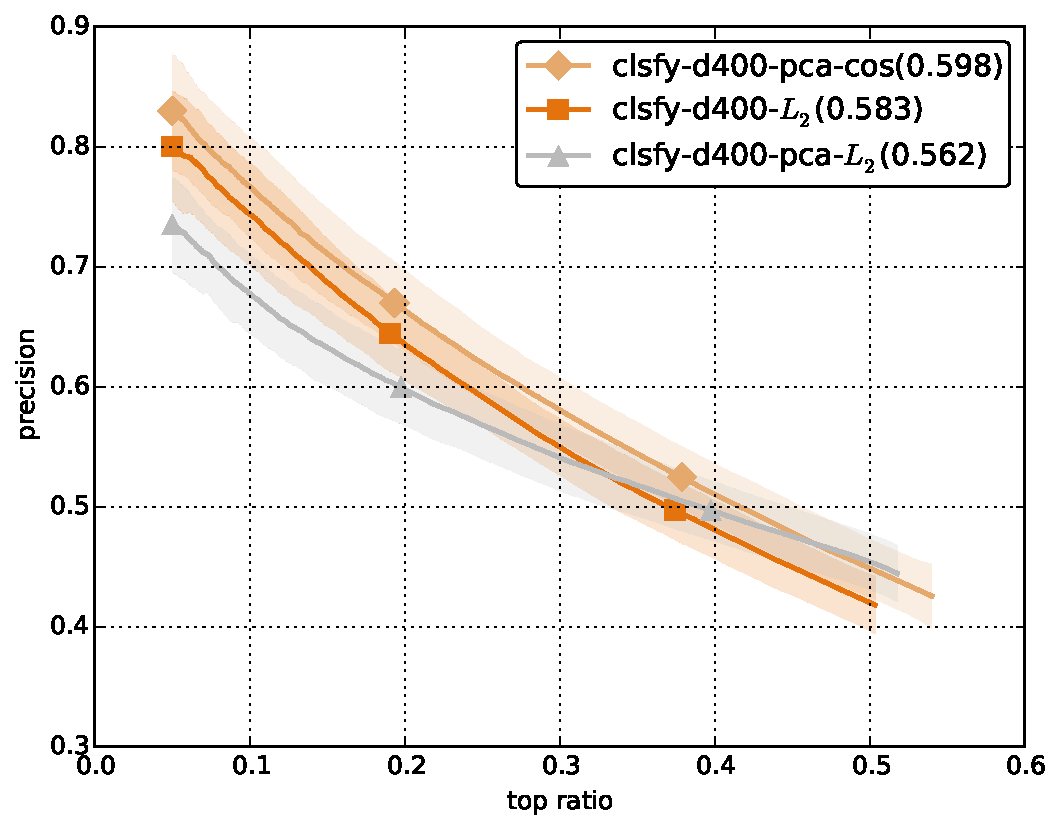
\includegraphics[width=0.6\textwidth]{res/expr/clsfy/pca/0.pdf}
    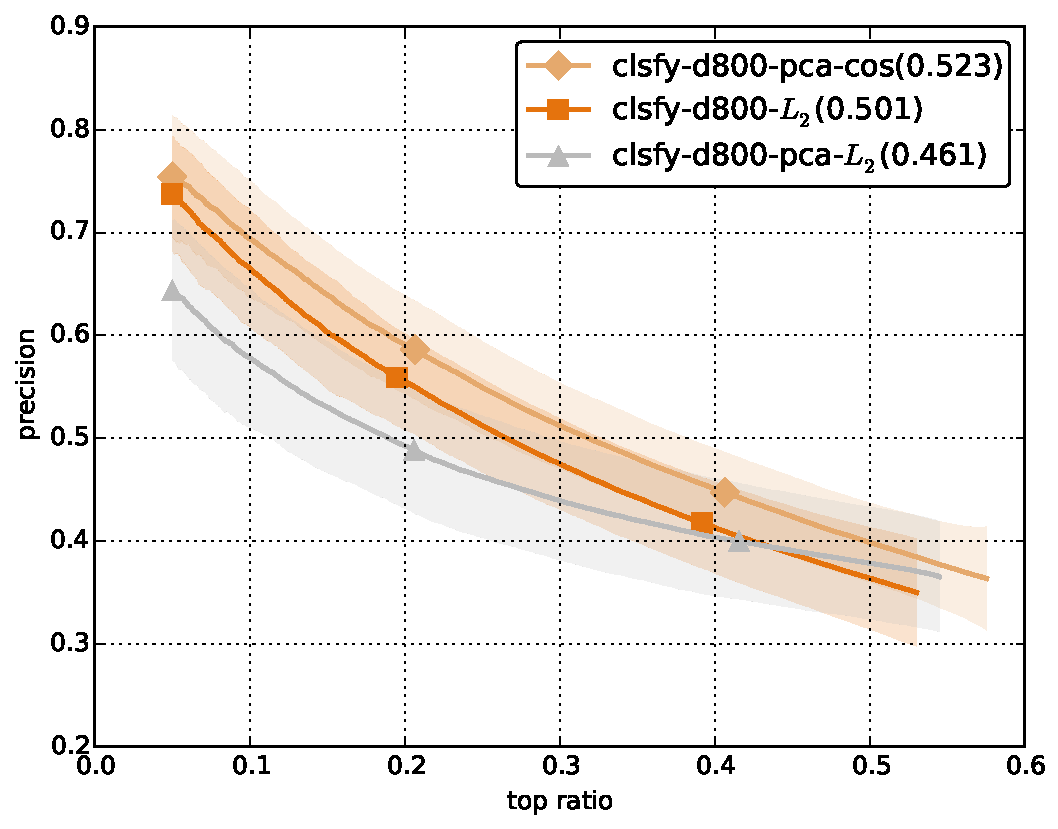
\includegraphics[width=0.6\textwidth]{res/expr/clsfy/pca/1.pdf}
    \caption{结合PCA提升多分类训练的深度卷积神经网络的特征性能}
    \label{fig:expr:curve:clsfy:pca}
\end{figure}


\subsection{基于度量学习进行特征学习的深度卷积神经网络}
我们采用了Adam\cite{kingma2014adam}来优化\secref{cnn:loss:mtrc}中定义的网络,
因为实验中我们发现其优化效果比SGD更好。与\secref{expr:clsfy}类似,
当学习速率自动下降到一定程度后停止训练。
在本小节中,我们将比较不同的参数选择对基于度量学习的网络所提取特征性能的影响。
关于曲线命名的具体法则,见\secref{expr:allresults}。

\subsubsection{距离度量}
由于训练时就直接使用了余弦距离,在测试时,
余弦距离的性能也应该比欧氏距离更好。
如\figref{expr:curve:mtrc:measure}所示,使用余弦距离时精确度的方差更小,
精确度普遍更高,而且最终顶峰比也更高。

\begin{figure}[H]
    \addtwocolplot{res/expr/mtrc/measure/0-0.pdf}{res/expr/mtrc/measure/0-1.pdf}
    \addtwocolplot{res/expr/mtrc/measure/1-0.pdf}{res/expr/mtrc/measure/1-1.pdf}
    \addtwocolplot{res/expr/mtrc/measure/2-0.pdf}{res/expr/mtrc/measure/2-1.pdf}
    \caption{不同距离度量下度量学习的深度卷积神经网络的特征性能}
    \label{fig:expr:curve:mtrc:measure}
\end{figure}

\subsubsection{损失函数中的$\delta$}
\eqnref{cnn:mtrc:loss}中用到了一个超参数$\delta$来控制对不同类的特征应有的距离。
我们实验了$\delta=0.5$和$\delta=0.65$两种设定,
发现虽然较大的$\delta$可以在训练集上让类内距离减小而类间距离增加,
但在测试集上却让性能有所下降。因此,控制$\delta$的值,
可以在一定程度上减轻过拟合。具体ROC曲线如\figref{expr:curve:mtrc:delta}所示,
其中带-mg的曲线表示使用了$\delta=0.65$。

\begin{figure}[H]
    \addtwocolplot{res/expr/mtrc/delta/0.pdf}{res/expr/mtrc/delta/1.pdf}
    \addplottcs{res/expr/mtrc/delta/2.pdf}
    \caption{$\delta$对度量学习的深度卷积神经网络的性能影响}
    \label{fig:expr:curve:mtrc:delta}
\end{figure}

\subsubsection{训练数据量}
我们也测试了不同训练数据量对最终性能的影响,发现数据量达到一定程度后,
并不会对最终性能产生太大影响,这也与预期相符。
ROC曲线见\figref{expr:curve:mtrc:datasize}。
\begin{figure}[H]
    \addtwocolplot{res/expr/mtrc/datasize/0.pdf}{res/expr/mtrc/datasize/1.pdf}
    \caption{训练数据量对度量学习的深度卷积神经网络的性能影响}
    \label{fig:expr:curve:mtrc:datasize}
\end{figure}

\subsubsection{结合PCA进一步提升性能}
与\secref{expr:clsfy:pca}中讨论的方法类似,
我们可以用PCA替代最后一层全连接来提升特征的性能。
然而我们发现,对某些网络,倒数第二层的一些神经元由于偏置量太大而始终没被激活,
导致PCA时很多特征值几乎为$0$,无法实现$50$维的PCA输出。
我们限制了PCA时最小特征值不小于0.1,并依次决定最终PCA的输出维度。
ROC曲线见\figref{expr:curve:mtrc:pca}。
\begin{figure}[H]
    \addtwocolplot{res/expr/mtrc/pca/0.pdf}{res/expr/mtrc/pca/1.pdf}
    \addplottcs{res/expr/mtrc/pca/2.pdf}
    \caption{结合PCA提升度量学习的深度卷积神经网络的特征性能}
    \label{fig:expr:curve:mtrc:pca}
\end{figure}


\subsection{结果汇总\label{sec:expr:allresults}}
在本小结中,我们将汇总所有结果,以备参考。

首先介绍结果命名规则。所有结果按照``方法名-[参数0-][参数1-]...距离度量''
的形式命名。距离度量包括cos和$L_2$,分别代表余弦距离和欧氏距离。
方法名包括ISA、clsfy、mtrc,分别代表层叠卷积ISA、
多分类训练的深度卷积神经网络和度量学习训练的深度卷积神经网络。
对于后两种方法,还有如下额外参数:
\begin{description}
    \item[d$N$] 表示训练数据量为从每个被试上随机采样$N$个图像块
    \item[mg] 表示基于度量学习的方法使用了$\delta=0.65$
    \item[pca] 表示使用了PCA代替最后一层全连接
    \item[o$N$] 表示最终特征维度不是$50$维,而是$N$维
\end{description}

我们将各类方法中,结果最好的ROC曲线共同绘制在\figref{expr:curve:all}里,
以便比较。为了便于观察,该图中没有绘制方差范围。

\begin{figure}[H]
    \addplot{res/expr/all.pdf}
    \caption{ROC曲线汇总}
    \label{fig:expr:curve:all}
\end{figure}

另外,我们将所有实验结果的一些统计数据放在\tabref{expr:all}中。
其中括号内标注的是按该列统计值的排名,前三名加粗标注。
\begin{longtable}{l|l|l|l|l|l}
    \caption{全部实验结果}
    \label{tab:expr:all} \\
    \tabtop
    {\heiti 名称} & {\heiti AUC} & {\heiti 平均精确度} & {\heiti 最大顶峰比} &
        {\heiti 最小精确度} & {\heiti 最大精确度} \\
    \tabmid
    ISA-cos&0.218 (25)&0.349 (32)&$\boldsymbol{0.674}$ {\bf (1)}&0.235 (33)&0.543 (28)\\
ISA-l2&0.122 (35)&0.212 (35)&$\boldsymbol{0.629}$ {\bf (2)}&0.179 (34)&0.227 (36)\\
clsfy-d200-cos&0.246 (18)&0.555 (12)&0.493 (29)&0.399 (19)&0.782 (7)\\
clsfy-d200-l2&0.247 (17)&0.571 (9)&0.483 (31)&0.405 (15)&0.788 (5)\\
clsfy-d400-cos&0.259 (14)&0.551 (13)&0.521 (25)&0.402 (16)&0.774 (8)\\
clsfy-d400-l2&0.264 (10)&0.583 (5)&0.503 (28)&0.418 (12)&$\boldsymbol{0.801}$ {\bf (3)}\\
clsfy-d400-pca-cos&$\boldsymbol{0.293}$ {\bf (2)}&0.598 (4)&0.540 (19)&0.426 (9)&$\boldsymbol{0.830}$ {\bf (1)}\\
clsfy-d400-pca-l2&0.263 (11)&0.562 (10)&0.518 (26)&0.445 (4)&0.735 (13)\\
clsfy-d800-cos&0.213 (26)&0.433 (28)&0.542 (18)&0.333 (29)&0.611 (22)\\
clsfy-d800-l2&0.241 (20)&0.501 (19)&0.530 (21)&0.350 (26)&0.738 (12)\\
clsfy-d800-pca-cos&0.275 (7)&0.523 (16)&0.575 (8)&0.364 (24)&0.755 (10)\\
clsfy-d800-pca-l2&0.228 (22)&0.461 (25)&0.545 (16)&0.365 (23)&0.644 (20)\\
clsfy-d2000-cos&0.156 (33)&0.313 (33)&0.548 (14)&0.266 (32)&0.363 (33)\\
clsfy-d2000-l2&0.178 (32)&0.357 (31)&0.550 (13)&0.267 (31)&0.422 (32)\\
clsfy-d5000-cos&0.125 (34)&0.223 (34)&0.611 (4)&0.095 (35)&0.245 (35)\\
clsfy-d5000-l2&0.118 (36)&0.209 (36)&$\boldsymbol{0.616}$ {\bf (3)}&0.094 (36)&0.249 (34)\\
mtrc-d800-cos&0.274 (8)&0.520 (17)&0.577 (7)&0.359 (25)&0.729 (14)\\
mtrc-d800-l2&0.206 (28)&0.398 (29)&0.567 (12)&0.343 (27)&0.517 (29)\\
mtrc-d5000-cos&$\boldsymbol{0.299}$ {\bf (1)}&0.576 (6)&0.569 (11)&0.402 (17)&0.797 (4)\\
mtrc-d5000-l2&0.241 (19)&0.487 (20)&0.545 (15)&0.396 (20)&0.646 (19)\\
mtrc-d5000-pca-o44-cos&0.289 (4)&$\boldsymbol{0.609}$ {\bf (3)}&0.525 (23)&0.442 (5)&0.744 (11)\\
mtrc-d5000-pca-o44-l2&0.227 (23)&0.476 (22)&0.528 (22)&0.425 (10)&0.555 (26)\\
mtrc-d10000-cos&0.283 (5)&0.574 (8)&0.543 (17)&0.413 (13)&0.774 (9)\\
mtrc-d10000-l2&0.223 (24)&0.480 (21)&0.514 (27)&0.411 (14)&0.591 (24)\\
mtrc-d10000-pca-o47-cos&0.262 (12)&$\boldsymbol{0.615}$ {\bf (2)}&0.476 (33)&$\boldsymbol{0.450}$ {\bf (3)}&0.787 (6)\\
mtrc-d10000-pca-o47-l2&0.193 (30)&0.456 (26)&0.473 (34)&0.431 (7)&0.492 (31)\\
mtrc-mg-d800-cos&0.261 (13)&0.468 (24)&0.607 (5)&0.340 (28)&0.606 (23)\\
mtrc-mg-d800-l2&0.204 (29)&0.387 (30)&0.578 (6)&0.325 (30)&0.557 (25)\\
mtrc-mg-d5000-cos&0.279 (6)&0.535 (14)&0.573 (9)&0.396 (21)&0.677 (18)\\
mtrc-mg-d5000-l2&0.228 (21)&0.475 (23)&0.531 (20)&0.387 (22)&0.643 (21)\\
mtrc-mg-d5000-pca-o47-cos&0.250 (16)&0.576 (7)&0.484 (30)&0.433 (6)&0.723 (15)\\
mtrc-mg-d5000-pca-o47-l2&0.190 (31)&0.440 (27)&0.482 (32)&0.400 (18)&0.512 (30)\\
mtrc-mg-d10000-cos&$\boldsymbol{0.291}$ {\bf (3)}&0.558 (11)&0.571 (10)&0.425 (11)&0.697 (17)\\
mtrc-mg-d10000-l2&0.253 (15)&0.534 (15)&0.525 (24)&0.429 (8)&0.723 (16)\\
mtrc-mg-d10000-pca-cos&0.269 (9)&$\boldsymbol{0.641}$ {\bf (1)}&0.470 (35)&$\boldsymbol{0.474}$ {\bf (1)}&$\boldsymbol{0.823}$ {\bf (2)}\\
mtrc-mg-d10000-pca-l2&0.211 (27)&0.506 (18)&0.467 (36)&$\boldsymbol{0.469}$ {\bf (2)}&0.553 (27)\\

    \tabbottom
\end{longtable}
% f}}}


\section{小结与讨论}
在本章中,我们先提出了仅依赖于对单个器官的分割标注的特征评测标准,
并详细报告了我们进行的各种实验在该评测标准上的性能。
总的来说,可以得到以下几点结论:
\begin{enumerate}
    \item 在监督信号中加入对不变性的先验要求的深度卷积神经网络所得到的特征,
        总体而言比完全非监督的层叠卷积ISA得到的特征性能要好很多;
    \item 不恰当的特征距离度量会导致性能严重恶化;
        我们仅实验了余弦距离和欧氏距离两种,发现对ISA、PCA及度量学习等方法,
        用余弦距离效果更好;对多分类学习,用欧氏距离效果更好;
    \item 基于多分类训练的网络对训练数据量有较严格的要求,
        过多或过少均会导致性能下降;
    \item 对于度量学习的网络,其损失函数中的$\delta$需要设置成合适的值,
        过大的$\delta$可能导致过拟合;
    \item 使用PCA替代深度卷积神经网络的最后一层全连接,在一定程度上可以提升性能
\end{enumerate}

% vim: filetype=tex foldmethod=marker foldmarker=f{{{,f}}}


